\begin{tikzpicture}
	\begin{axis}[
		axis lines=middle,
		axis equal,
		xmin=-4,
		xmax=4,
		ymin=-4,
		ymax=4,
		xlabel=$z_1$,
		ylabel=$z_2$,
		axis background/.style={fill=gray!50}
	]
		\addplot[-, purple, line width=4pt] coordinates {({ln(1/3)}, -5) ({ln(1/3)}, 5)} node[below, left, pos=0.9] {$\ln\left( \dfrac{1}{3} \right)$};
		\addplot[-, blue, line width=4pt] coordinates {({ln(2/3)}, -5) ({ln(2/3)}, 5)} node[below, left, pos=0.2] {$\ln\left( \dfrac{2}{3} \right)$};
		\addplot[-, black!70!green, line width=4pt] coordinates {(0, -5) (0, 5)} node[below, right, pos=0.2] {$0$};
		\addplot[-, black!50!green, line width=4pt] coordinates {({ln(2)}, -5) ({ln(2)}, 5)} node[below, left, pos=0.9] {$\ln(2)$};
		\addplot[-, green, line width=4pt] coordinates {({ln(3)}, -5) ({ln(3)}, 5)} node[below, right, pos=0.2] {$\ln(3)$};
		
		\addplot[-, yellow, line width=4pt] coordinates {(-5, {5/6*pi}) (5, {5/6*pi})} node[below, left, pos=0.1] {$\dfrac{5}{6}\pi$};
		\addplot[-, orange, line width=4pt] coordinates {(0, {1/3*pi}) (5, {1/3*pi})} node[below, left, pos=0.7] {$\dfrac{1}{3}\pi$};
		\addplot[-, red, line width=4pt] coordinates {(-5, 0) (0, 0)};
		\addplot[-, black!50!red, line width=4pt] coordinates {(-5, {-1/3*pi}) (0, {-1/3*pi})} node[below, left, pos=0.7] {$-\dfrac{1}{3}\pi$};
		\addplot[-, purple, line width=4pt] coordinates {(-5, {-5/6*pi}) (5, {-5/6*pi})} node[below, right, pos=0.7] {$\dfrac{5}{6}\pi$};
	\end{axis}
\end{tikzpicture}